\documentclass[16pt, a4paper]{report}


\title{Gravitational Wave Astronomy}
\author{To be updated}
\date{\today}


\usepackage{amsmath}
\usepackage{tensor}
\usepackage{gensymb}
\usepackage[utf8]{inputenc}
\usepackage{graphicx}

\begin{document}
\maketitle

\pagebreak
Abstract here
\pagebreak

\pagebreak
\section{Introduction}
add general relativity work here
add spacetime work here
add history of gw work here
add explanation of gw here
\pagebreak

\pagebreak

\section{Linearized theory of Gravitational waves}

Einstein's field equations 
\begin{equation}
    G_{\mu\nu}= \frac{8 \pi  G}{c^{4}}  T_{\mu\nu}
\end{equation}
is a tensor equation which describes gravity in form of Einstein's tensor, $G_{\mu\nu}$ which is directly dependent on the geometry of space-time which is altered by the stress-energy tensor $T_{\mu\nu}$

Another field equation that relates the geometry or curvature of space-time to stress-energy tensor is 

\begin{equation}
    R_{\mu\nu}-\frac{1}{2}g_{\mu\nu}R=\frac{8\pi G}{c^{4}}T_{\mu\nu}
\end{equation}
where $R_{\mu\nu}$ is the Riemann tensor which describes the curvature of space-time, $R$ is the scalar curvature and $g_{\mu\nu}$ is the gravitational field tensor.

Any change in matter distribution will be recorded in in $T_{\mu\nu}$. So if $T_{\mu\nu}$ changes then according to equation 2, gravitational field tensor $g_{\mu\nu}$ also has to change. 

If $h_{\mu\nu}$ is the variation induced in space-time then the new gravitational field tensor $\tilde{g}_{\mu\nu}$ is given by 

\begin{equation}
    \tilde{g}_{\mu\nu} = g_{\mu\nu} + h_{\mu\nu}
\end{equation}

To get the new gravitational field, Einstein's field equation should be solved for $\tilde{g}_{\mu\nu}$ which gives 

\begin{equation}
    \tilde{h}_{\mu\nu} = h_{\mu\nu} - \frac{1}{2} \, \eta_{\mu\nu} \, h^{\alpha}_{\alpha}
\end{equation}
 where $\eta_{\mu\nu}$ is the gravity where space is flat i.e. $\eta_{\mu\nu} = g_{\mu\nu}$ and $h^{\alpha}_{\alpha}$ is summed for all spatial coordinates i.e. $\alpha$ takes values $(1,2,3) $ which corresponds to $(x,y,z)$.
 
 The admitted solutions for this variations in space time $\tilde{h}_{\mu\nu}$ has solution in the form of 
 
 \begin{equation}
     \tilde{h}_{\mu\nu} = A^{\mu\nu}\, e^{ik_{\alpha}x^{\alpha}}
 \end{equation}
 
 which is a 3D wave equation where $A^{\mu\nu}$ is the Amplitude tensor, $i = \sqrt{-1} $, $k_{\alpha} = (k_{x},k_{y},k_{z})$ is the wave vector and $x^{\alpha} = (x^{1},x^{2},x^{2}) = (x,y,z)$ is the position vector.
\pagebreak

\section{Properties of Gravitational waves}
The amplitude tensor $A^{\mu\nu}$ has two forms $A^{\mu\nu}_{+}$ and $A^{\mu\nu}_{\times}$ which are orthogonal to each other. They can be represented as 

\begin{equation}
    A^{\mu\nu}_{+} = h_{+}\, \varepsilon^{\mu\nu}_{+}
\end{equation}

\begin{equation}
    A^{\mu\nu}_{\times} = h_{\times} \,\varepsilon^{\mu\nu}_{\times}
\end{equation}

where $\varepsilon^{\mu\nu}_{+}$ and $\varepsilon^{\mu\nu}_{\times}$ are unit polarization tensors.

\begin{equation}
\varepsilon^{\mu\nu}_{+} =
\begin{bmatrix}
0 & 0 & 0 & 0 \\
0 & +1 & 0 & 0 \\
0 & 0 & -1 & 0 \\
0 & 0 & 0 & 0 \\
\end{bmatrix}
\end{equation}
\\
\begin{equation}
\varepsilon^{\mu\nu}_{\times} =
\begin{bmatrix}
0 & 0 & 0 & 0 \\
0 & 0 & +1 & 0 \\
0 & +1 & 0 & 0 \\
0 & 0 & 0 & 0 \\
\end{bmatrix}
\end{equation}

\noindent In general relativity any tensor with indices $\mu\nu$ is a rank 2 tensor with 4 rows and 4 columns where each index can take values of space time coordinates which are $(t,x,y,z)$ , and position of each element is associated with any two coordinates. Thus in such tensors, the positions of elements are associated with space-time as follows:

\begin{equation*}
    \begin{bmatrix}
    tt & tx & ty & tz \\
    xt & xx & xy & xz \\
    yt & yx & yy & yz \\
    zt & zx & zy & zz \\
    \end{bmatrix}
\end{equation*}

So when we compare the unit polarization tensors $\varepsilon^{\mu\nu}_{+}$ and $\varepsilon^{\mu\nu}_{\times}$ with the above one, we see that in $\varepsilon^{\mu\nu}_{+}$ the non zero entries are +1 in $`xx$' direction and -1 in $`yy$' direction, hence the $A^{\mu\nu}_{+}$ amplitude is oriented only along X and Y axes, thus this gravitational wave which oscillates along X and Y axes is called as `PLUS' polarized wave because the vibration resembles `+' symbol. But in $\varepsilon^{\mu\nu}_{\times}$ the non zero entries are +1 in $`xy$' direction and -1 in $`yx$' direction, hence the $A^{\mu\nu}_{+}$ amplitude is oriented in the `XY' plane at a an angle of 45$\degree$ to the axes, thus this gravitational wave which oscillates in the `XY' plane at a an angle of 45$\degree$ to the axes is called as `CROSS' polarized wave because the vibration resembles `$\times$' symbol. 
\\

So the equation of polarized gravitational waves are:-\\
(+) wave $\Rightarrow $  $\tilde{h}_{\mu\nu} = h_{+}\, \varepsilon^{\mu\nu}_{+}\, e^{i(\omega t - k_{z}z)}$\\
$(\times)$ wave $\Rightarrow $  $\tilde{h}_{\mu\nu} = h_{\times}\, \varepsilon^{\mu\nu}_{\times}\, e^{i(\omega t - k_{z}z)}$ \pagebreak
\subsection{Effect of Gravitational waves on objects}
\subsubsection{Plus polarized effect}
When a plus polarized wave passes through the object, since such gravitational wave makes space-time oscillate in X and Y axes only. So the points in space along axis will come close during compression and go far during stretching. Thus the object itself will be compressed and stretched along the axes, perpendicular to the direction of propagation of wave.

\subsubsection{Cross polarized effect}
When a cross polarized wave passes through the object, since such gravitational wave makes space-time oscillate along the line which makes an inclination of 45$\degree$ with X and Y axes (i.e. along the line $x=y$ and $x=-y$). So the points in space along those line will come close during compression and go far during stretching. Thus the object itself will be compressed and stretched along those lines, perpendicular to the direction of propagation of wave.
\\

Thus for every phase difference of $\pi/2$ we get the shape of object to be as follows
when a plus polarized wave passes and a cross polarized wave passes through a spherical object:

\begin{center}
    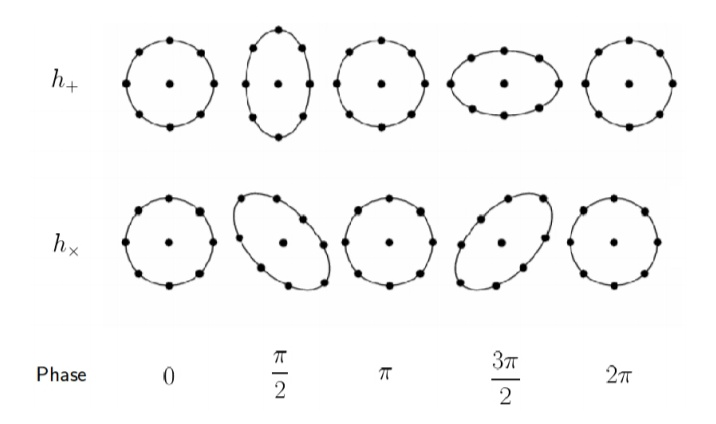
\includegraphics[scale=0.5]{images.tex/effect_of_gw.jpeg}
\end{center}
 \pagebreak
\subsection{Energy transported by gravitational wave}

Since gravitational wave travels in the speed of light, the energy is also transported at that speed. And since Energy flux is equal to the product of Energy and speed, The average energy flux `$E$' is given by

\begin{equation}
    E = \frac{c^{3}}{16\pi G} \left \langle (h_{+})^{2} + (h_{\times})^{2} \right \rangle 
\end{equation}

So we see the energy flux is very huge because of the term $\frac{c^{3}}{16 \pi G}$ which is in the order of $10^{33}$ Joules sec/ metre$^2$  and it also depends on the average of the square of the plus and cross polarized amplitudes `$h_{+}$' and `$h_{\times}$'. \\

Due to such huge energy it carries the wave can travel unimpeded forever through space and no obstacle can damp gravitational wave because the space in which the obstacle lies itself is the medium of the wave. But the Doppler effect and decrease in amplitude due to radiation of energy causes the wave to die out after the wave travels a very long distance according to the relation $A \propto \frac{1}{r^2}$\:. So the power or intensity of gravitational wave decreases as it moves through space according to this inverse square law. 

\begin{figure}[h]
    \centering
    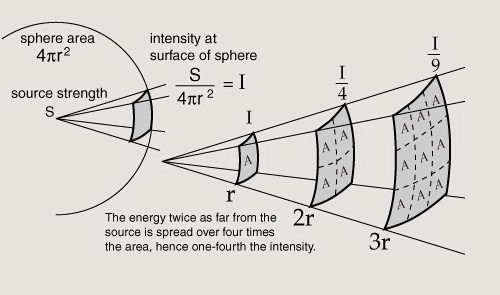
\includegraphics[scale=0.915]{images.tex/inverse_square.jpeg}
    \caption{ Here we see how the intensity of wave changes as it goes farther from the source according to the inverse square law.\\
    \textbf{Source :-} http://www.mysearch.org.uk/website1/html/339.Laws.html}
\end{figure} \pagebreak

\section{Sources of Gravitational waves}
Theory of general relativity predicts that gravitational waves can be generated by any dynamically changing system containing moving objects by producing radiation-reaction forces in their source i.e. waves will be generated and carries the exact rate of energy which is extracted from the source.   
\subsection{Single accelerating object in space}
 Accelerating objects like pulsars can create gravitational wave. According to general relativity, mass creates stress in space-time and thus can change the geometry of it by bending and changing the curvature. Then if this object moves, then the curvature also moves along with it. But if the object accelerates in space-time in a circular manner, then the ripples will be created in space-time which is which radiates gravitational waves. This is similar to creation of water waves when we move our finger in a circular fashion in water. So higher the mass of object and it's acceleration, stronger is the gravitational wave it produces.
 
 Such continuously spinning bodies produces continuous gravitational waves, where it's nature is sinusoidal for a longer period of time. This happens only if spin rate of this object is constant. Such gravitational waves have same frequency and amplitude, but they are not yet discovered.\\


\begin{figure}[h]
    \centering
     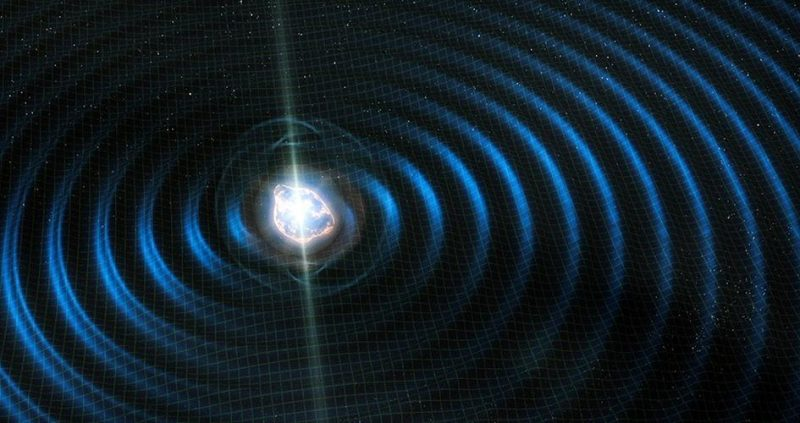
\includegraphics[height = 9cm, width = 12cm]{images.tex/continuous_gw.jpg}
    \caption{Computer simulation of Continuous gravitational wave by a pulsar \\
    \textbf{Source :-} https://earthsky.org/space/gravitational-waves-single-neutron-stars-planck-einsteinhome}
\end{figure}

\subsection{Revolving Binary Systems}

Revolving binary systems are formed when two massive objects orbit around their common centre of mass called barycenter. Such systems create gravitational waves by a mechanism called `Inspiral'. There are four phases in this mechanism. \\

\textbf{Interlocking phase} :- This the longest phase where the bodies come closer and get interlocked by their gravity and start to revolve each other around the barycentre. \\

\textbf{Spiral phase} :- Here the objects start getting close as they revolve. Due to the decrease in the distance between them the orbital energy is decreased and this energy is radiated as gravitational wave. But as they come closer and closer, they loose more and more energy, thus the intensity of gravitational wave increases.\\

\textbf{Merger phase} :- During this phase, the bodies collide by producing immense gravitational waves and merge. \\

\textbf{Ring-down phase} :- Finally, the merged bodies become stable and the gravitational wave intensity decreases exponentially and they stop producing gravitational waves. \\

Revolving binary systems produce Burst gravitational waves. This is because the intensity of gravitational waves increases logarithmically during interlocking phase, and exponentially during the spiral phase, then it reaches a peak in merger phase, and finally it decreases rapidly to zero during ring-down phase. The detectors are capable of recording the signal only for a small range of frequency, So in this wave form, the frequency comes to the detecting range and rapidly goes out of range. Thus the signal strength suddenly increases and stops like a burst.

\begin{figure}[h]
    \centering
    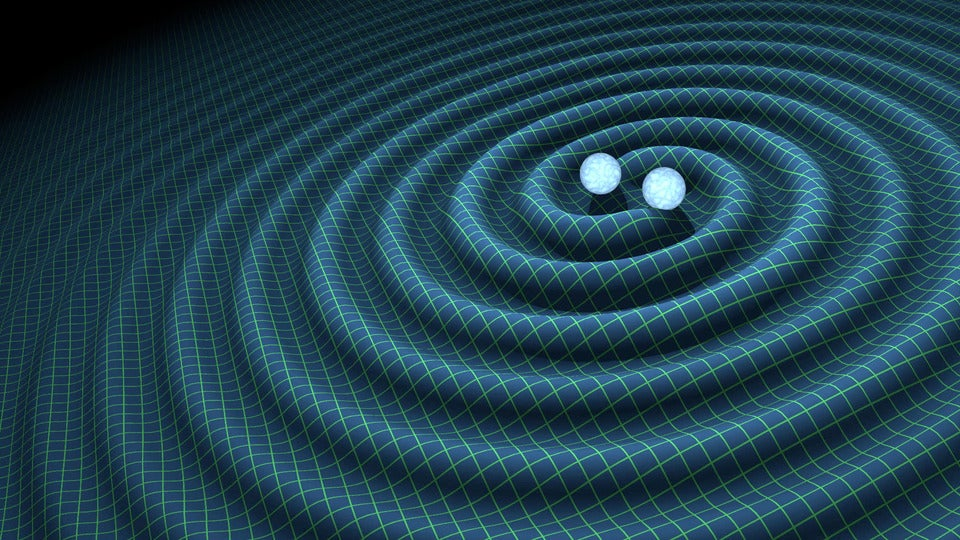
\includegraphics[height = 5.585cm, width = 12 cm]{images.tex/binaries.jpeg}
    \caption{Two massive bodies in inspiral mechanism creating gravitational waves \\
    \textbf{Source :-} https://www.scientificamerican.com/article/gravitational-waves-discovered-from-colliding-black-holes1/}
\end{figure}

\pagebreak

\subsubsection{Binary Black Holes (BBH)}

Black holes are massive objects that can warp space-time extensively. If two black holes get closer and start the inspiral mechanism ,they create ripples in space-time and radiate gravitational waves. Such gravitational waves were the first ones to be detected by LIGO in 2015, September 14th. It was estimated that the collision occurred 1.3 billion years ago, thus the merger occurred 1.3 billion light-years away. This merger was named as `\textbf{GW150914}' meaning Gravitational Wave on 15/09/14. This signal lasted for about half a second.

\subsubsection{Binary Neutron Stars (BNS)}

Neutron stars are dense stars formed by the remnants when a massive star explodes as Supernova. So when two neutron stars merge through inspiral mechanism, they can radiate gravitational waves. First BNS merger was detected on 17th August 2017 and this was named as `\textbf{GW170817}', where the merger was analyzed both by Electromagnetic waves (Gamma ray) and gravitational waves. The signal lasted for comparatively longer duration for about 100 seconds, thus the mass was estimated to be lesser than black holes and was recognised as neutron star merge.



\begin{figure}[h]
   \begin{minipage}{0.6\textwidth}
     \centering
     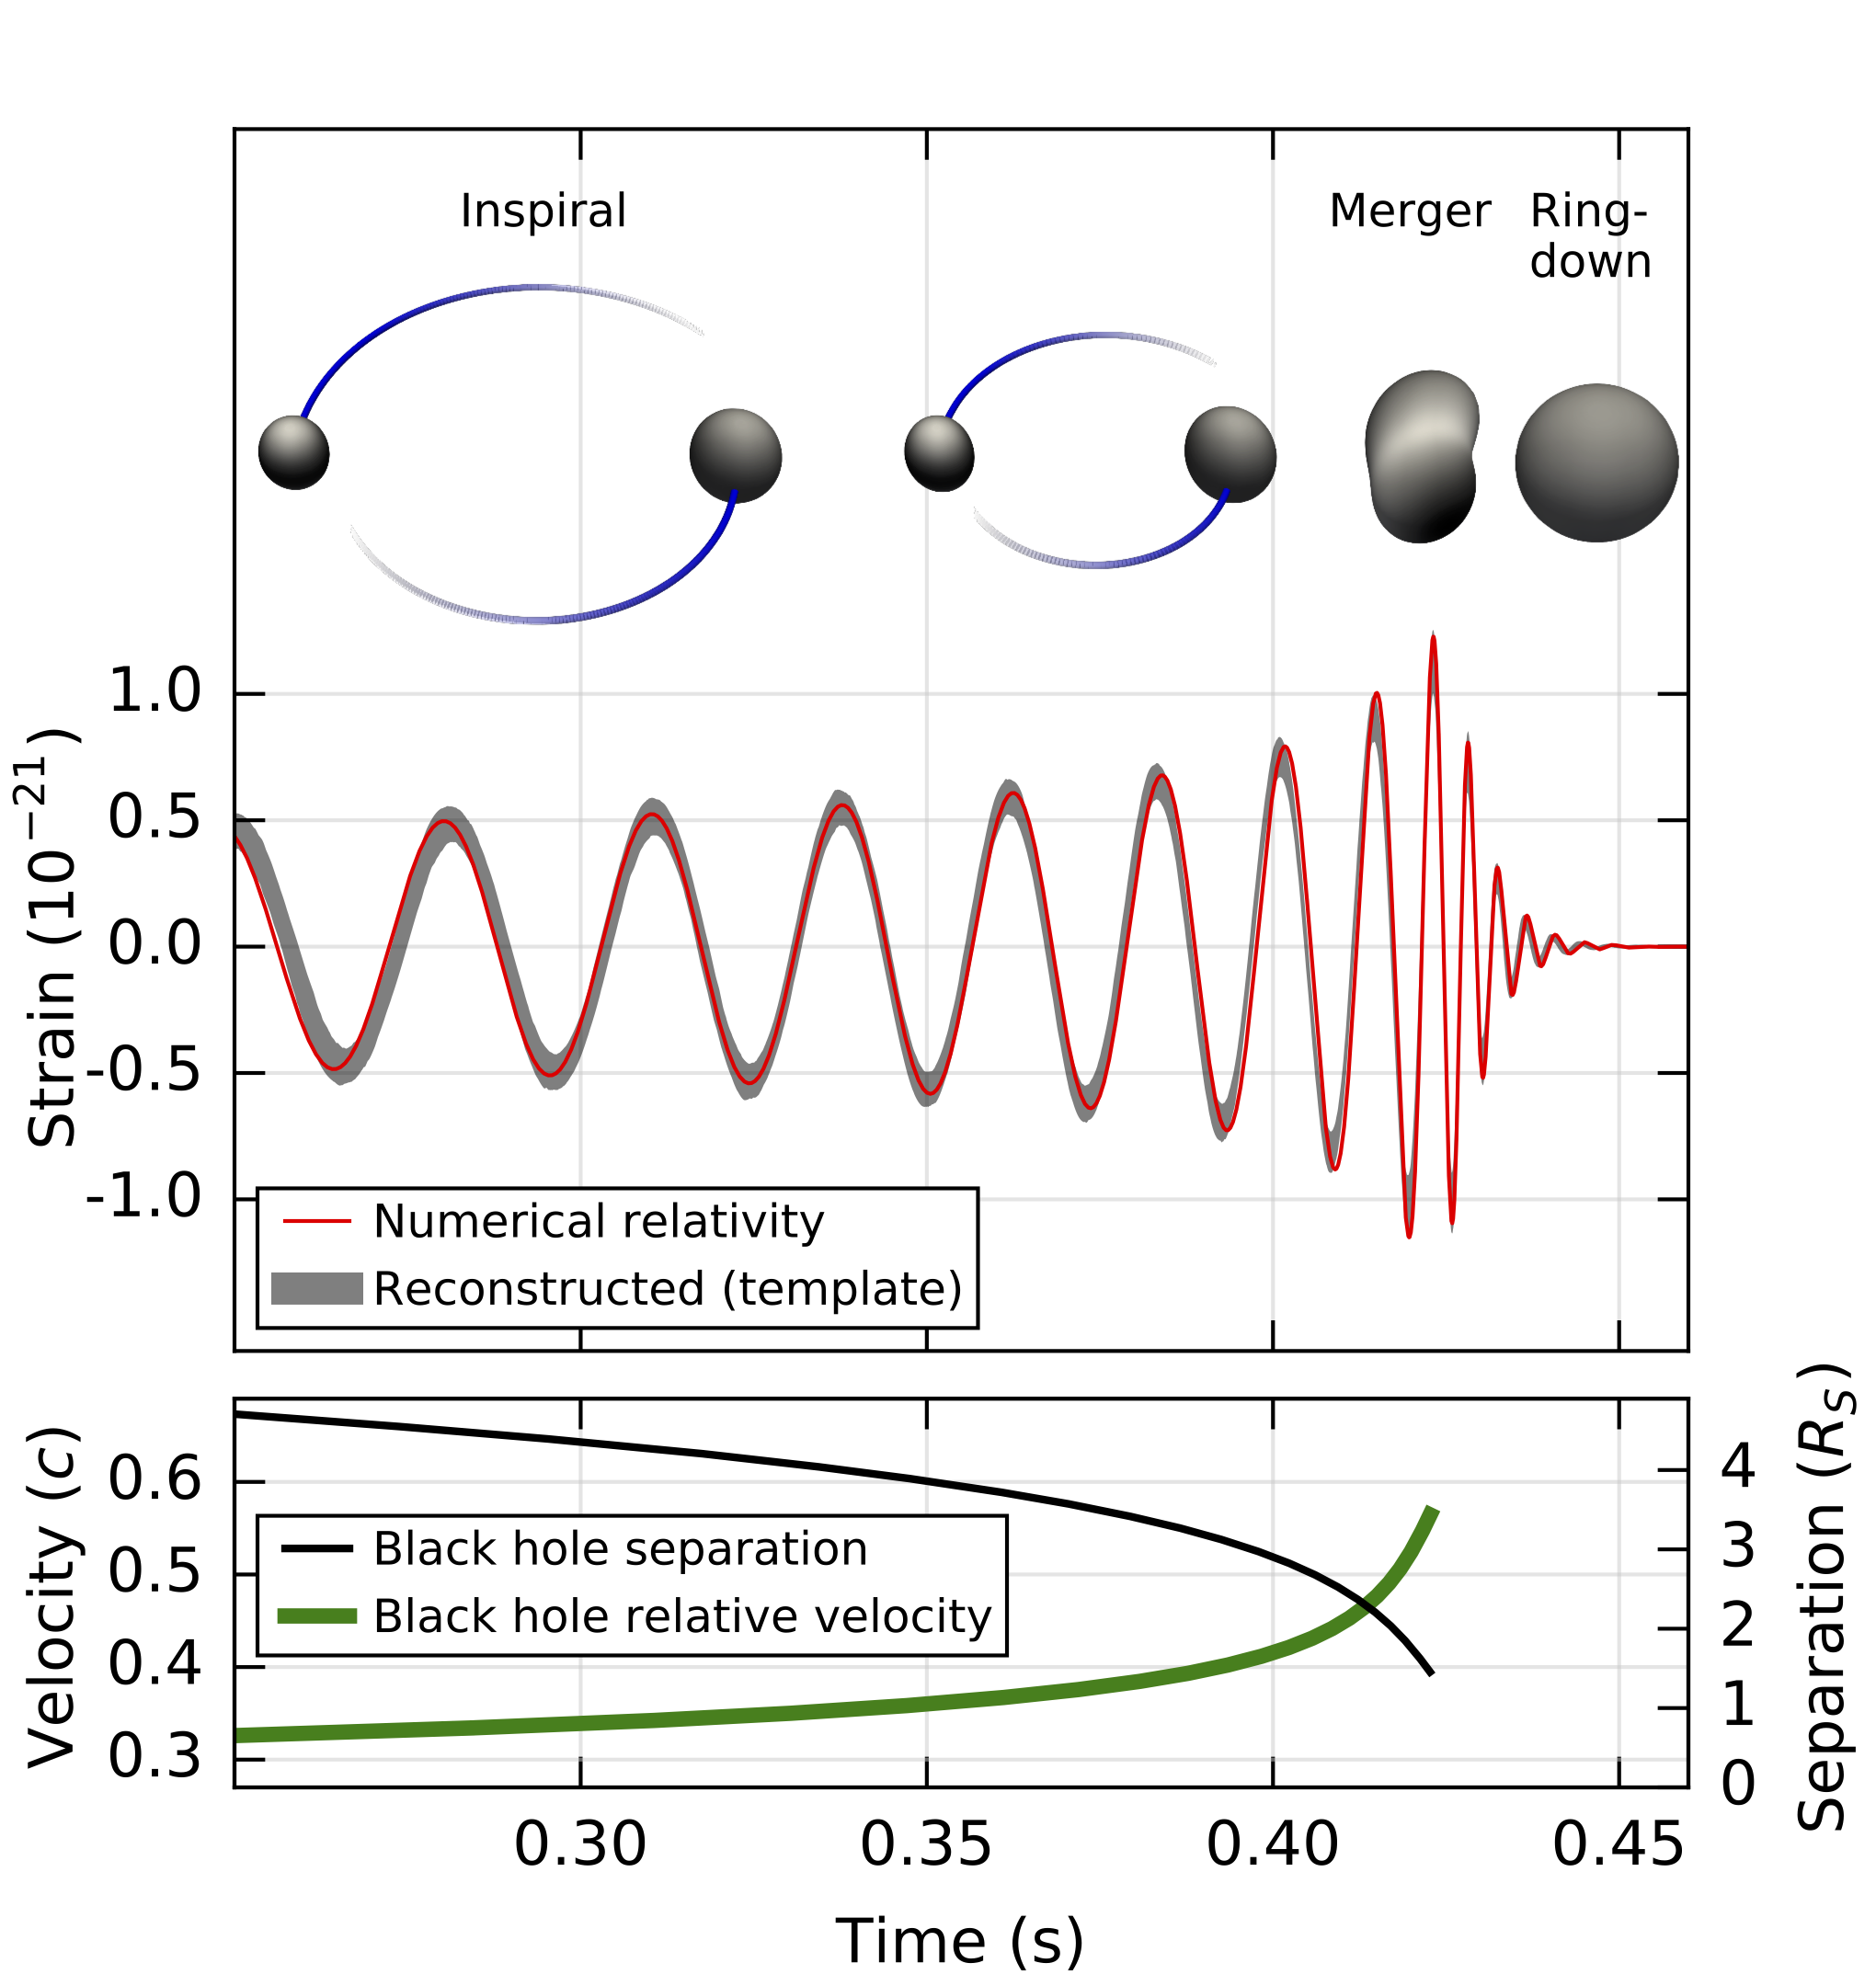
\includegraphics[height = 7cm , width  4 cm]{images.tex/GW150914.png}
     \caption{Characteristics of GW150914\\ Source - https://www.ligo.org/science/}
   \end{minipage}\hfill
   \begin{minipage}{0.6\textwidth}
     \centering
     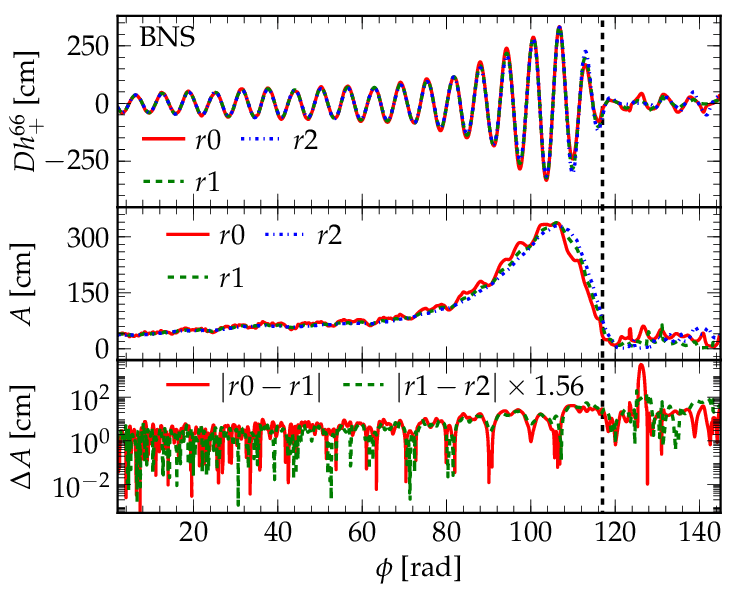
\includegraphics[height = 7cm ,width = 8 cm]{images.tex/GW170817.png}
     \caption{Characteristics of GW170817\\ Source - https://www.researchgate.net/233846764}
   \end{minipage}
\end{figure}

%add your work in form of folders and use \input{folder_name.tex/file_name}

\end{document}
